\documentclass[times, utf8, seminar, numeric]{fer}
\usepackage{booktabs}
\usepackage{url}
\usepackage[section]{placeins}

\begin{document}

% Ukljuci literaturu u seminar
\nocite{*}

\title{Poboljšanje djelomično sastavljenog genoma dugim očitanjima}

\author{Bruno Kovač, Tonko Sabolčec, Fabijan Čorak}

\voditelj{doc. dr. sc. Krešimir Križanović}

\maketitle

\tableofcontents

\chapter{Uvod}
Sekvenciranje genoma svodi se na kombiniranje očitanja u jednu cjelinu. Ovaj rad pretpostavlja da su očitanja već sastavljena, ali djelomično - u fragmente. Jedan takav fragment naziva se \textit{contig}. Dakle, zadatak se svodi na što bolje povezivanje \textit{contiga}, što smo učinili postupkom opisanim u \cite{Du345983}. Taj rad definira nekoliko mjera preklopljenosti očitanja koje kombiniraju duljinu područja \textit{overlap} ($OL$), \textit{overhang} ($OH$) i \textit{extension} ($EL$). Mjere su ovdje definirane za dva očitanja $S_1$ i $S_2$; pripadnost područja određena je indeksom.

\begin{figure}[h]
	\centering
	\centerline{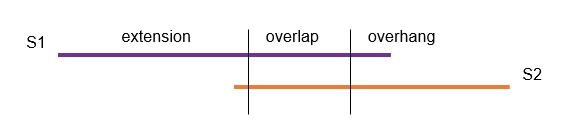
\includegraphics[width=0.6\linewidth]{img/overlap}}
	\caption[]{Preklop dvaju očitanja s naznačenim područjima}
	\label{fig:overlap}
\end{figure}

\begin{itemize}
	\item \textit{sequence identity ($SI$)} - omjer ukupnog broja podudarajućih znakova u \textit{overlap} područjima i duljine duljeg od tih dvaju područja
		\[ SI = \frac{\text{broj\_podudaranja}}{\max(OL_1, OL_2)} \]
	\item \textit{overlap score ($OS$)}
		\[ OS = \left(OL_1 + OL_2\right)\frac{SI}{2} \]
	\item \textit{extension score ($ES$)} - uz $S_2$ kao produžetak od $S_1$
		\[ ES_2 = OS + \frac{EL_2 - OH_1 - OH_2}{2} \]
\end{itemize}


\chapter{Postupak}
Sastavljanje očitanja u niz modelirano je izgradnjom i obilaskom grafa.
\section{Izgradnja grafa}
Svaki \textit{contig} i svako očitanje čine jedan čvor grafa. Dodatno, u skup čvorova dodaje se i reverzna inačica svakog očitanja i \textit{contiga} jer nije unaprijed poznato koja je pogodna orijentacija. Čvor koji predstavlja \textit{contig} zovemo \textit{anchor}. Za svako očitanje 
Brid postoji između svaka dva čvora čiji je $SI$ veći od nekog minimuma. Pritom svaki brid nosi informacije o preklopljenosti čvorova koje povezuje ($SI$, $OS$, $ES$). Te mjere računaju se na temelju informacija o preklopljenosti dobivenih korištenjem alata \textit{minimap2} opisanog u \cite{minimap2}.

\section{Obilazak grafa}

\begin{figure}[h]
	\centering
	\centerline{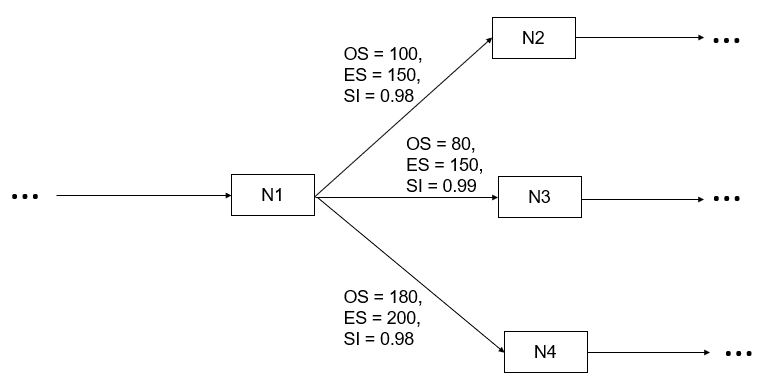
\includegraphics[width=0.6\linewidth]{img/traversal}}
	\caption{Odabir sljedećeg čvora u obilasku}
	\label{fig:traversal}
	\small
	Slika razmatra grananje u hipotetskom čvoru N1. Prvim postupkom prioritetna lista je: [N4, N2, N3], a drugim postupkom: [N4, N3, N2]. Treći postupak daje vjerojatnosti odabira čvorova \{N2: 150/500, N3: 150/500, N4: 200/500\}.
\end{figure}

\noindent
Kroz graf se traže putovi čije su krajnje točke \textit{anchor} čvorovi. Za to se koriste tri načina obilaska, prilikom kojih je postavljena maksimalna dubina pretraživanja i pamte se obiđeni čvorovi:
\begin{enumerate}
	\item Iz \textit{anchor} čvora pretraga se nastavlja u sve susjedne čvorove. Iz svakog sljedećeg čvora, pretraga se nastavlja u onaj susjed s kojim je najveći \textit{overlap score}, a kojim se u konačnici dolazi do \textit{anchor} čvora. Ako je \textit{overlap score} jednak, gleda se \textit{sequence identity}. Ako je pak i ta mjera jednaka, gleda se duljina očitanja.
	\item Kao i prethodni način, ali umjesto mjere \textit{overlap score} gleda se \textit{extension score}.
	\item U svakom čvoru susjed se odabire probabilistički - s vjerojatnošću odabira proporcionalnom mjeri \textit{extension score}, sve dok se ne dosegne \textit{anchor}. Postupak se pokreće iz svakog \textit{anchor} čvora proizvoljan broj puta. Ovo je tzv. Monte Carlo metoda.
\end{enumerate}

\section{Obrada putova}
Nakon agregacije putova dobivenih opisanim postupcima, odbacuju se duplikati i obrađuju se putovi između svaka dva \textit{anchor} čvora. Putovi se sortiraju uzlazno prema duljini i razmatraju se prozori fiksne širine $W$. Pritom $i$-ti prozor obuhvaća sve putove čija je duljina $L$: $(i-1)W < L \le iW$ za dobro definirane $i$. Koliko je koji prozor frekventan vidljivo je na primjeru povezivanja dvaju \textit{contiga} na slici \ref{fig:distribution}. Pretpostavka je da dominacija nekog prozora ukazuje na to da su u njemu putovi koji su izgledni kandidati za povezivanje dvaju \textit{anchor} čvorova između kojih se nalaze. Problem je što to ne mora biti istina, tj. moguće je dominiranje nekog prozora, a da ta dva \textit{anchor} čvora uopće nisu uzastopna.

\begin{figure}[h]
	\centering
	\centerline{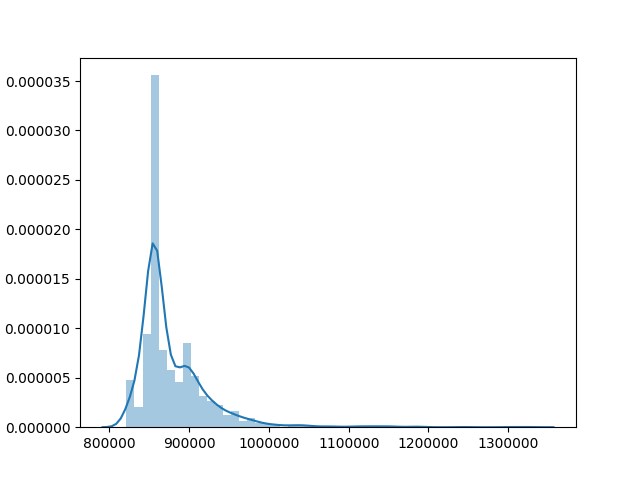
\includegraphics[width=0.6\linewidth]{img/distribution}}
	\caption{Dstribucija putova po prozorima fiksne širine}
	\label{fig:distribution}
	\small
	Distribucija putova između dva \textit{anchor} čvora. Na x-osi označene su širine prozora, a na y-osi frekventnost (udio brojnosti putova prozora u ukupnom broju putova). Najviši stupac dat će i reprezentant povezanosti dvaju čvorova.
\end{figure}

Za svaki par \textit{anchor} čvorova računa se konsenzus - struktura podataka koja sadrži reprezentativni put te broj valjanih putova između tih dvaju čvorova. Kao reprezentant odabire se proizvoljni čvor maksimalne duljine. Na slici \ref{fig:distribution} to je jedan od putova duljine cca 850000 (najviši stupac). Dodatno, iz susjedstva svakog \textit{anchor} čvora uklanjaju se oni \textit{anchor} čvorovi do kojih je broj putova ispod neke određene granice. Drugim riječima, takvi susjedi vjerojatno ne trebaju biti povezani. U konačnici se konstruiraju poboljšani sljedovi \textit{contiga} i za svako poboljšanje generira se izlazna datoteka. (OVDI DODAT KAKO SE KONSTRUIRAJU POBOLJŠANI SLJEDOVI)% TODO

\begin{figure}[h]
	\centering
	\centerline{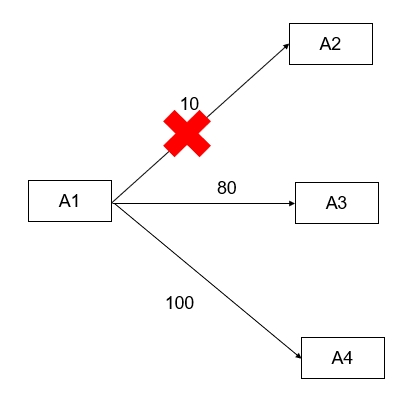
\includegraphics[width=0.6\linewidth]{img/valid_path_numbers_filtered}}
	\caption{Otpadanje jedne grane u slučaju kada je granica za odbacivanje 12.5\% od najvećeg broja valjanih putova.}
	\label{fig:validpathnumbersfiltered}
\end{figure}

\chapter{Rezultati}
Implementacija je ispitana na skupovima E. coli, C. jejuni i B. grahamii na jednoj dretvi uz procesorsku moć od ... GHz. Priložene su matrice preklapanja između referentnih skupova te prvo neobrađenih, a odmah zatim i obrađenih \textit{contiga}. Za svaki skup podataka prikazana su moguća poboljšanja sastavljanja \textit{contiga}. Sve matrice dobivene su alatom \textit{Gepard} opisanim u \cite{gepard}. Ishodište je u gornjem lijevom kutu, x-os predstavlja referencu, a y-os predstavlja \textit{contige}. Crne točke označavaju podudaranja. Predznak u opisima matrica označava korištenu orijentaciju \textit{contiga}: + je izvorna, a - reverzna. Npr. +5, -2 znači da je pronađeno povezivanje za izvorno orijentirani \textit{contig} 5 i reverzni 2.

\section{Generirani podaci}
Implementacija je ispitana i na umjetno generiranom skupu podataka.

\begin{figure}[h]
	\centering
	\centerline{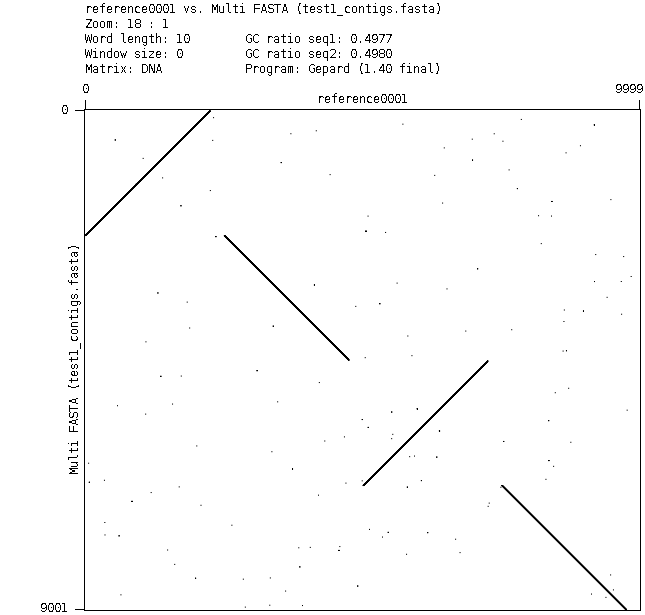
\includegraphics[width=0.6\linewidth]{img/generated}}
	\caption{Matrica preklapanja neobrađenih umjetno generiranih \textit{contiga} i točne reference.}
	\label{fig:generated}
\end{figure}

\begin{figure}[h]
	\centering
	\centerline{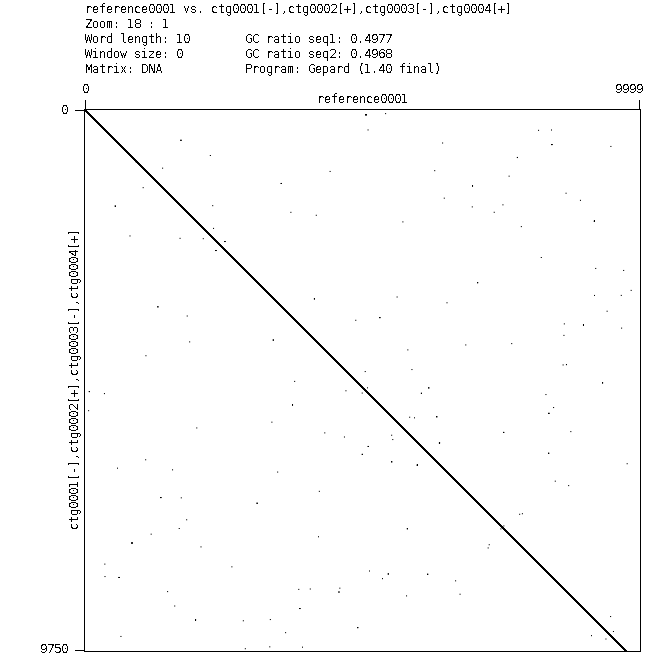
\includegraphics[width=0.6\linewidth]{img/generated_reference}}
	\caption{Poboljšanje generiranog testnog slučaja.}
	\label{fig:generatedreference}
	\small
	Pronađeni redoslijed \textit{contiga} je -1, +2, -3, +4.
\end{figure}



\section{E. coli}
Ovo je sintetski skup podataka, shodno čemu su i ostvareni rezultati bolji u usporedbi s narednim dvama, realnim skupovima. Rezultirajući izlazi programa zapravo su inverzi jedan drugog.

\begin{figure}[h]
	\centering
	\centerline{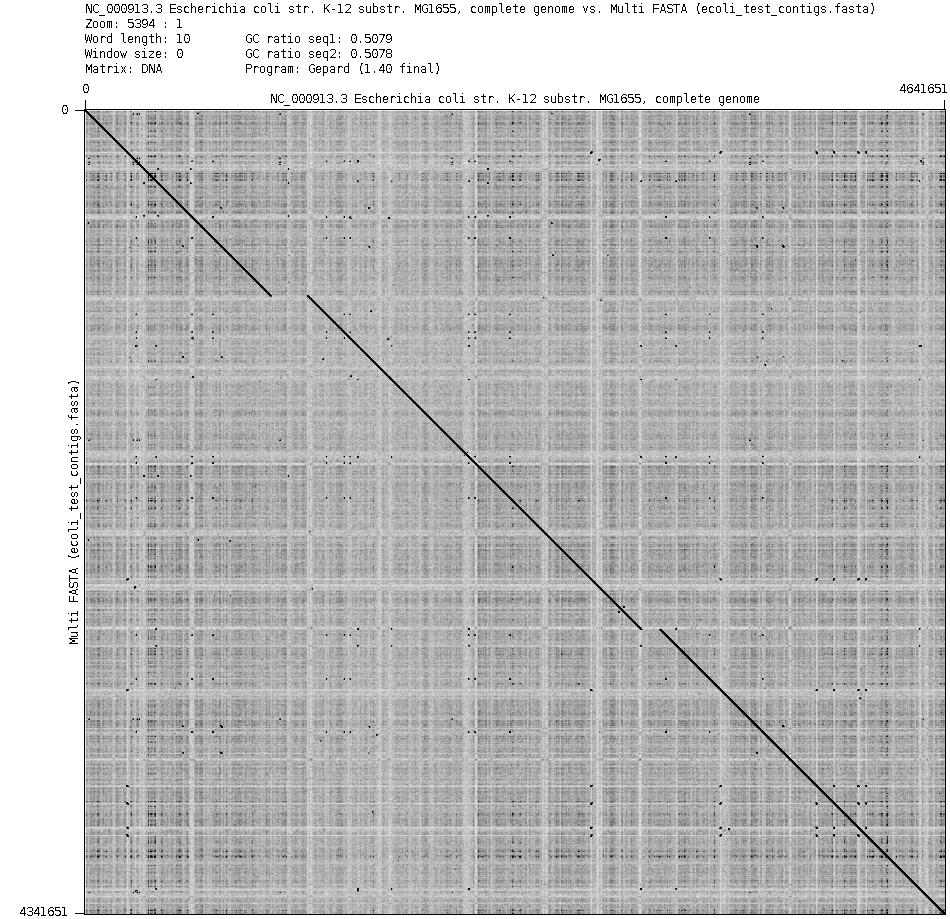
\includegraphics[width=0.6\linewidth]{img/ec_contigs}}
	\caption{Matrica preklapanja neobrađenih \textit{contiga} E. coli i referentnog skupa.}
	\label{fig:eccontigs}
\end{figure}

\begin{figure}[h]
	\centering
	\centerline{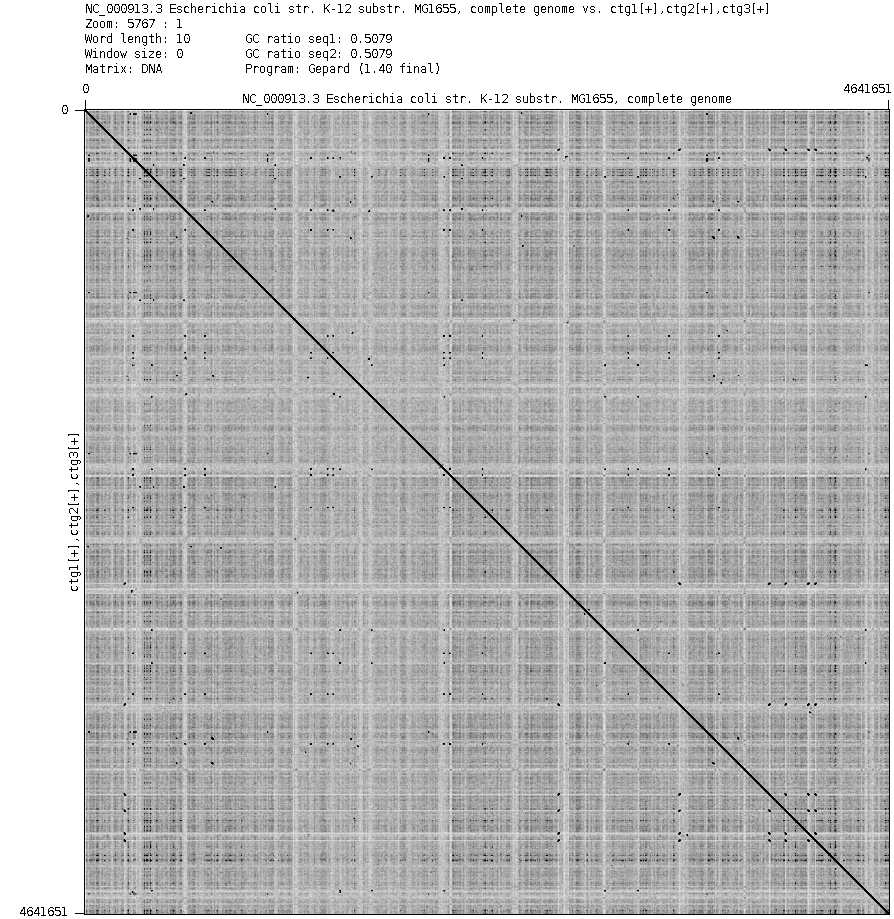
\includegraphics[width=0.6\linewidth]{img/ec_1_2_3}}
	\caption{Prvo poboljšanje: niz \textit{contiga} +1, +2, +3.}
	\label{fig:ec123}
\end{figure}

\begin{figure}[h]
	\centering
	\centerline{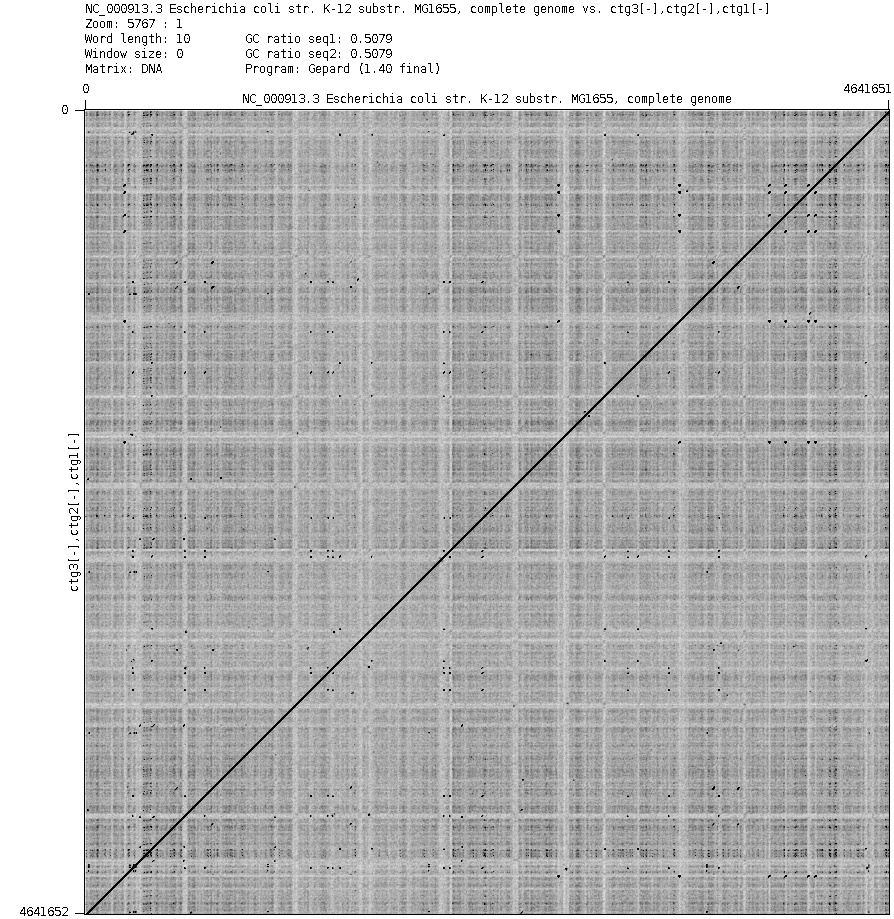
\includegraphics[width=0.6\linewidth]{img/ec_3_2_1_neg}}
	\caption{Drugo poboljšanje: niz \textit{contiga} -3, -2, -1.}
	\label{fig:ec321neg}
\end{figure}

\section{C. jejuni}
Prvi realni skup podataka predstavlja očitanja nad genomom bakterije C. jejuni.

\begin{figure}[h]
	\centering
	\centerline{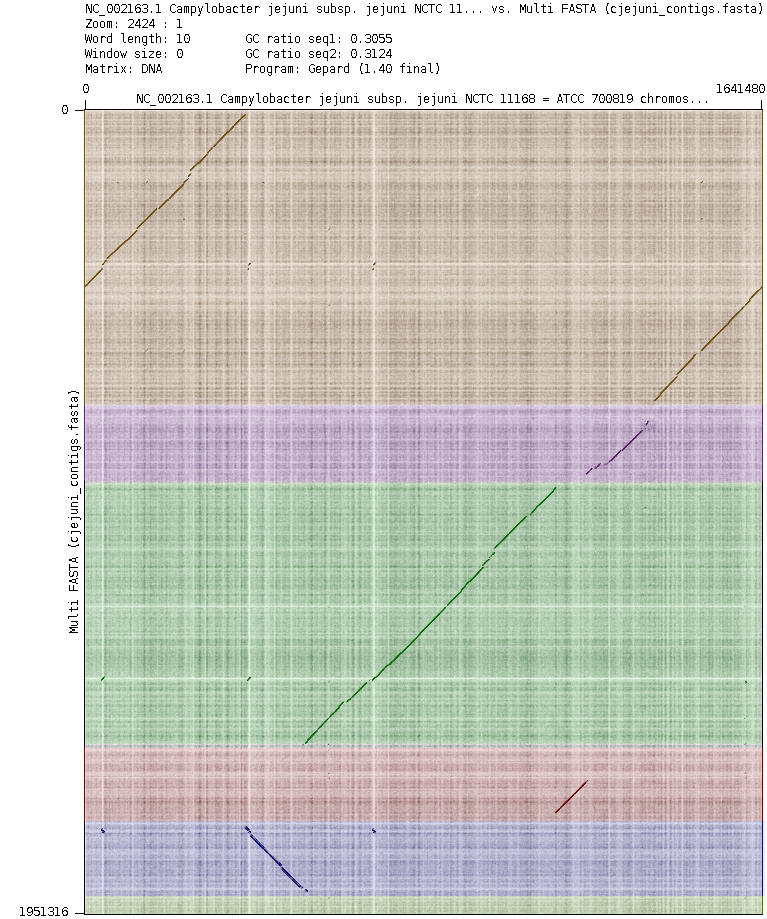
\includegraphics[width=0.6\linewidth]{img/cj_contigs}}
	\caption{Matrica preklapanja neobrađenih \textit{contiga} C. jejuni i referentnog skupa.}
	\label{fig:cjcontigs}
	\small
	Svaki contig predstavljen je jednom bojom. \textit{Contig} 1 (najgornji) već je dakle u ulaznoj datoteci definiran \textit{izlomljeno}, tj. obuhvaća očitanja sa stvarnog početka i kraja.
\end{figure}

\begin{figure}[h]
	\centering
	\centerline{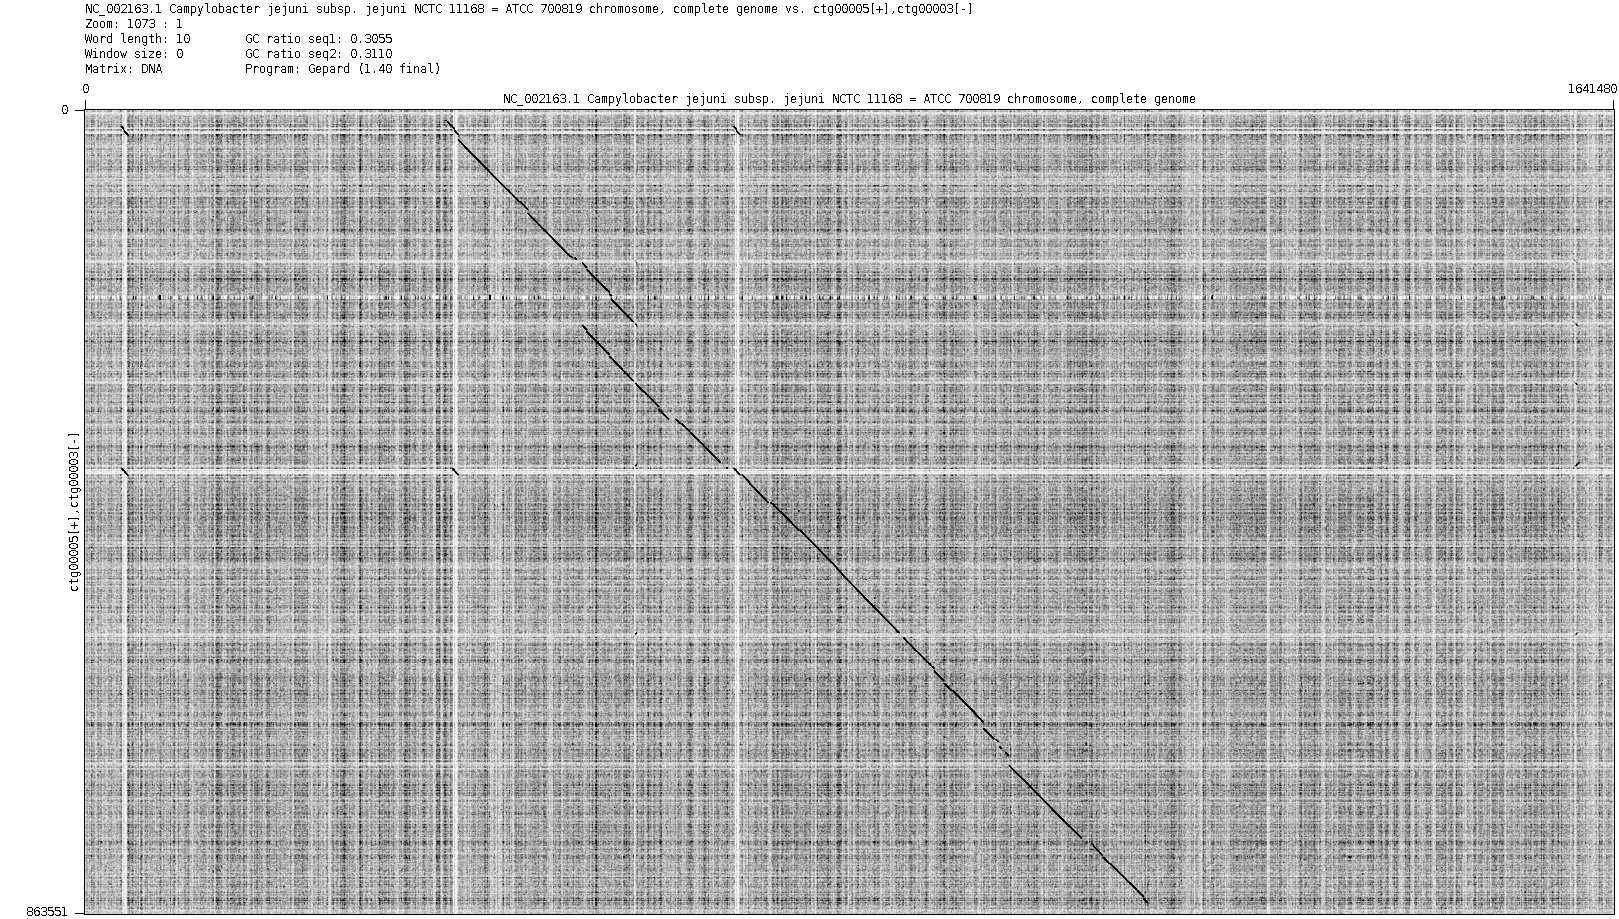
\includegraphics[width=0.6\linewidth]{img/cj_5_3}}
	\caption{Poboljšanje: niz \textit{contiga} +5, -3.}
	\label{fig:cj53}
\end{figure}

\section{B. grahamii}
Drugi realni skup podataka čine očitanja genoma bakterije B. grahamii.

\begin{figure}[h]
	\centering
	\centerline{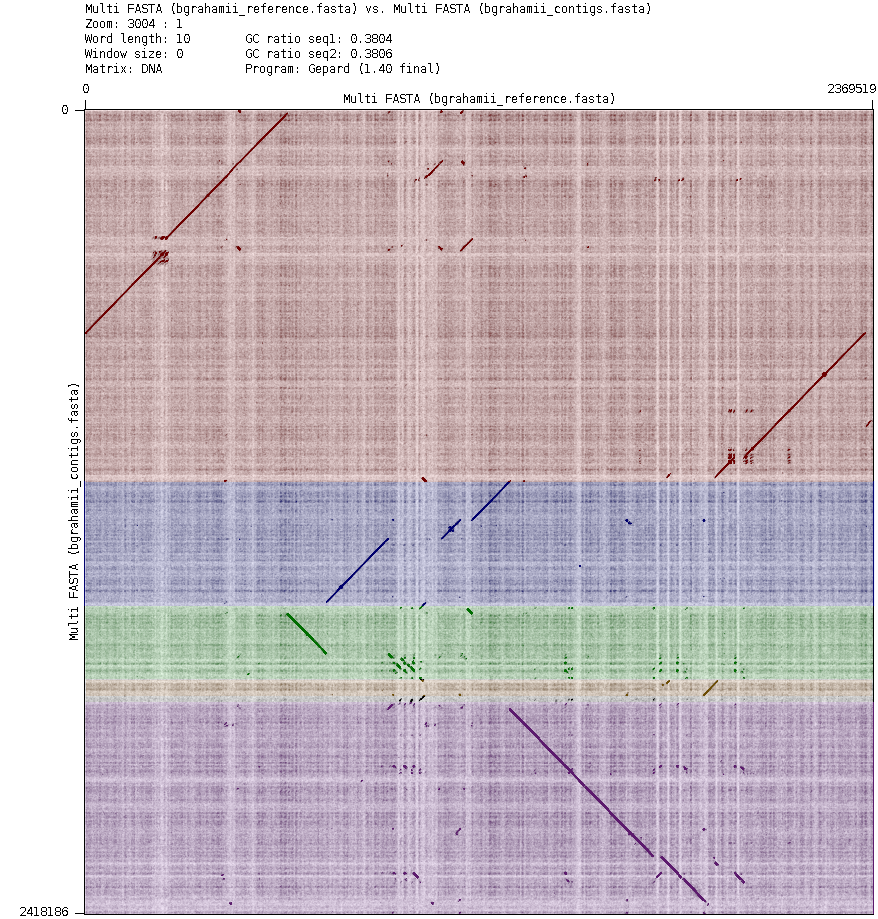
\includegraphics[width=0.6\linewidth]{img/bh_contigs}}
	\caption{Matrica preklapanja neobrađenih \textit{contiga} B. grahamii i referentnog skupa.}
	\label{fig:bhcontigs}
	\small
	Svaki contig predstavljen je jednom bojom. Ponovno su vidljive izlomljenosti u ulaznim podacima.
\end{figure}

\begin{figure}[h]
	\centering
	\centerline{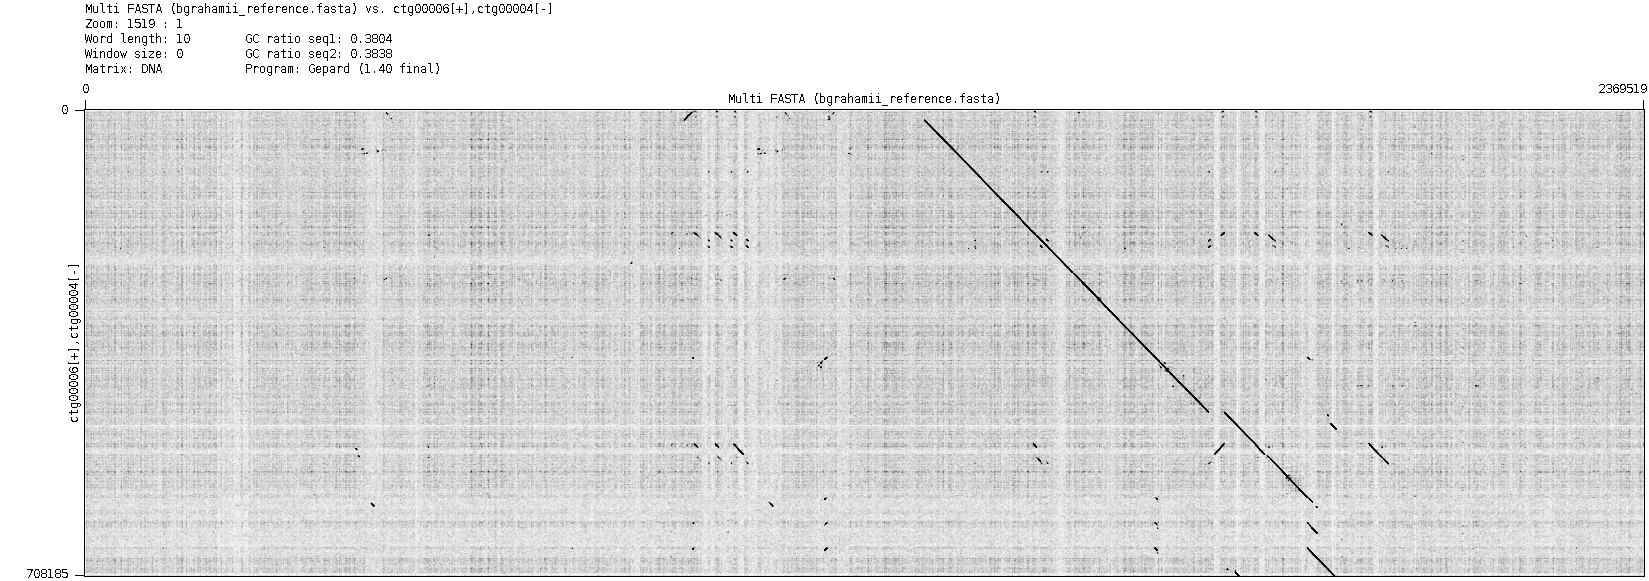
\includegraphics[width=0.6\linewidth]{img/bh_6_4}}
	\caption{Poboljšanje: niz \textit{contiga} +6, -4.}
	\label{fig:bh64}
\end{figure}

\begin{figure}[h]
	\centering
	\centerline{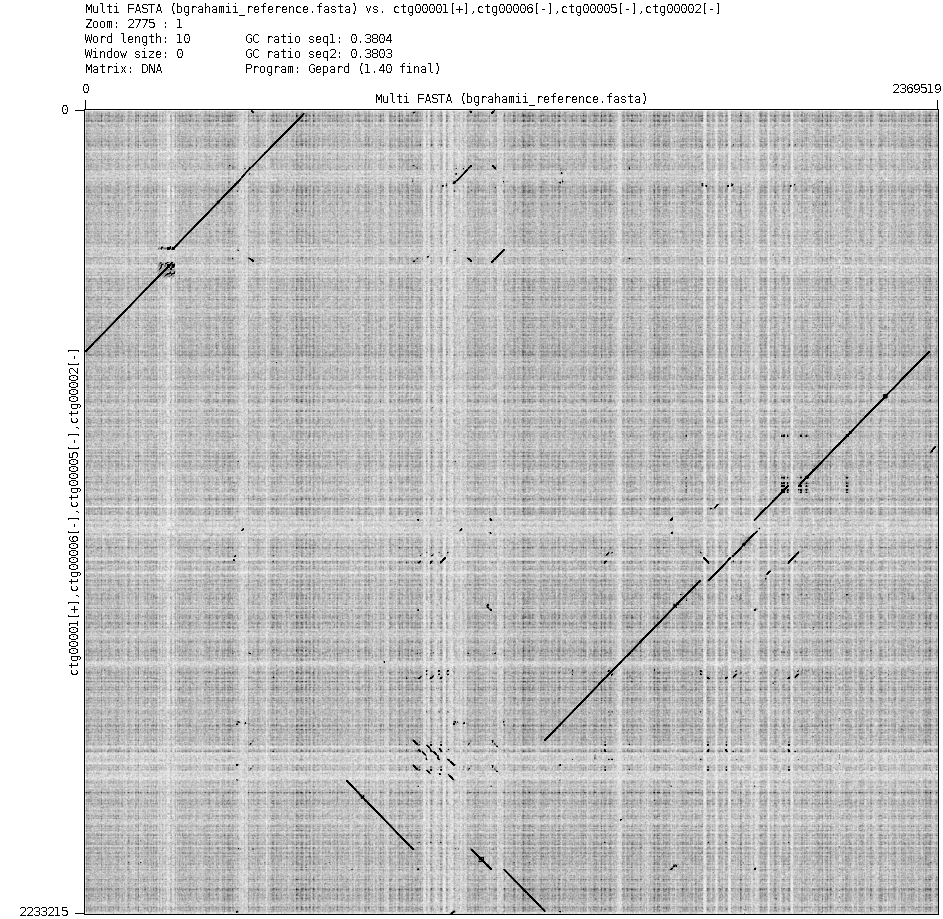
\includegraphics[width=0.6\linewidth]{img/bh_1_6_2}}
	\caption{Poboljšanje: niz \textit{contiga} +1, -6, -5, -2.}
	\label{fig:bh162}
\end{figure}

\section{Vremensko i memorijsko opterećenje}

\begin{center}
\begin{tabular}[h]{|c||c|c|}
	\hline
	skup podataka & vrijeme (s) & memorija (GiB)\\
	\hline
	\hline
	E. coli & X & Y \\
	\hline
	C. jejuni & B & C \\
	\hline
	B. grahamii & W & Z \\
	\hline
\end{tabular}
\end{center}

\chapter{Zaključak}
Implementacija uspijeva pronaći poboljšane nizove \textit{contiga}, s većom uspješnošću za sintetski primjer E. coli koji nema dubioznih \textit{contiga} 

\bibliography{literatura}
\bibliographystyle{fer}

\end{document}
